\documentclass[../resumosTCOM.tex]{subfiles}

\newenvironment{conditions}
  {\par\vspace{\abovedisplayskip}\noindent\begin{tabular}{>{$}l<{$} @{${}={}$} l}}
  {\end{tabular}\par\vspace{\belowdisplayskip}}

\begin{document} 

FA não determinista:
\begin{itemize}
    \item Pode estar em mais do que um estado ao mesmo tempo.
    \item A partir de um estado, com um input, pode ir para vários estados.
    \item No final, basta que um dos etados alcançados seja o estado final.
\end{itemize}

\paragraph{}

\(NFA = (Q, \sum, \delta, q_0, F)\)
\begin{itemize}
    \item Igual ao DFA, exceto que a função de transição \(\delta\) retorna um sub-conjunto de Q, em vez de um único estado.
    \item Tabela de transição usa conjuntos de estados.
        \begin{figure}[H]
            \centering
            \subfloat{{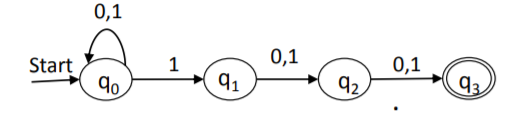
\includegraphics[width=5cm]{images/nfa.PNG} }}%
            \qquad
            \subfloat{{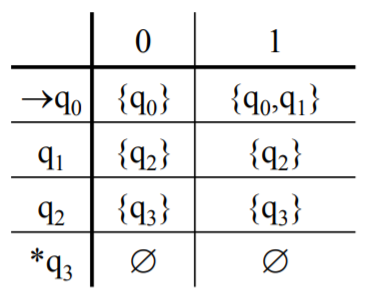
\includegraphics[width=5cm]{images/nfa_table.PNG} }}%
            \label{fig:nfa}%
        \end{figure}
        \[NFA \quad A = (\{q_0, q_1, q_2, q_3\}, \{0, 1\}, \delta, q_0, \{q_3\})\]
        \[\delta(q_0, 0) = \{q_0\}\]
        \[\delta(q_0, 1) = \{q_0, q_1\}\]
        \[\delta(q_1, 0) = \{q_2\}\]
        \[\delta(q_1, 1) = \{q_2\}\]
        \[\delta(q_2, 0) = \{q_3\}\]
        \[\delta(q_2, 1) = \{q_3\}\]
        \[\delta(q_3, 0) = \emptyset\]
        \[\delta(q_3, 1) = \emptyset\]
    \item Para converter um NFA num DFA usa-se a técnica de construção de subconjuntos: se o NFA tem n estados, o DFA terá, no máximo, \(2^n\) estados, incluindo o estado morto (\(\emptyset\)).
\end{itemize}

\paragraph{}

Estado morto (Dead State) é um estado de não aceitação com auto-transições para todos os símbolos do alfabeto. É usado para capturar erros num DFA.

\end{document}

